% !TEX program = pdflatex
% ============================================================
% GRETSI 2027 — Historical session — SHORT VERSION (24 slides)
% "Semantic segmentation in remote sensing"
% after M. Pastorino, G. Moser, J. Zerubia
% (../../article/Martina_TSI_GRETSI_segmentation_semantique.pdf).
%
% English version of ../main.tex: same theme, same content, same
% 24 slides. The only deliberate differences are the language and the
% broken citation of slide 9, which is fixed here (see README.md).
%
% Tightened version of the talk: 6 sections instead of 11, 20 talk
% slides, no section slides, no back-up credits slide. Reduced
% bibliography (54 entries, journals and conferences abbreviated).
%
% Build: make  (latexmk + pdfLaTeX + biber, theme in theme/)
% ============================================================
\documentclass[svgnames,9pt,aspectratio=169]{beamer}

\usepackage[english]{babel}
\usepackage{csquotes}
\usepackage{amsmath,amssymb,amsfonts,mathtools}
\usepackage{graphicx}
\usepackage{booktabs}
\usepackage{tikz}
\usetikzlibrary{positioning, shapes, arrows.meta, calc, fit, backgrounds, babel}

% ------------------------------------------------------------
% The theme tests the \draftmode primitive. LuaTeX provides it; pdfTeX
% has only known it since TeX Live 2024 (it was \pdfdraftmode before).
% This alias lets the file compile with either engine.
% ------------------------------------------------------------
\makeatletter
\ifdefined\draftmode\else
  \ifdefined\pdfdraftmode
    \let\draftmode\pdfdraftmode
  \else
    \providecommand{\draftmode}{0}%
  \fi
\fi
\makeatother

% ------------------------------------------------------------
% Inria 2024 Beamer theme (theme/ directory, unmodified).
% ------------------------------------------------------------
\usetheme{inria}
\renewcommand{\thankyou}{Thank you for your attention.}

% ------------------------------------------------------------
% Bibliography: the order of the .bib file is the order of the paper.
% \nocite{*} appears at the start of the document so that the [n]
% numbers on the slides follow that order.
% ------------------------------------------------------------
\usepackage[backend=biber,style=numeric,sorting=none,
            maxbibnames=4,minbibnames=3,giveninits=true,
            doi=false,isbn=false,url=false,eprint=false]{biblatex}
\addbibresource{references.bib}
\renewcommand*{\bibfont}{\tiny}
\setlength{\bibitemsep}{0.35ex}

% ------------------------------------------------------------
% Università di Genova logo (the Inria theme allows for one logo only).
% textpos coordinates: fractions of \paperwidth / \paperheight.
% ------------------------------------------------------------
\newcommand{\logounige}[1][0.185]{%
  \begin{textblock}{#1}[1,0](0.955,0.085)
    
\includegraphics[width=\textwidth]{imgs/logos/logo_orizzontale_COLORE}
  \end{textblock}}

% ------------------------------------------------------------
% Formatting commands
% ------------------------------------------------------------
% Emphasis
\newcommand{\hl}[1]{\textcolor{inria-rouge}{\textbf{#1}}}

% Inline bibliographic pointer: [n] in grey
\newcommand{\refc}[1]{\,\textcolor{gris_fonce_inria}{\footnotesize\cite{#1}}}

% Short caption under a figure (centred)
\newcommand{\legende}[1]{%
  \par\vspace{0.4ex}{\scriptsize\color{gris_fonce_inria}\centering #1\par}}

% Credit / copyright: in the flow, right below the sub-captions (centred)
\newcommand{\credit}[1]{%
  \par\vspace{0.35ex}{\tiny\color{gris_fonce_inria}\centering #1\par}}

% Full references cited on the slide, at the very bottom.
% Compact format: at most two authors, no volume, no number, no pages.
\newtoggle{brefcite}
\AtEveryCitekey{\iftoggle{brefcite}%
  {\clearfield{pages}\clearfield{volume}\clearfield{number}}{}}
\newcommand{\bibline}[1]{%
  \par\hangindent=1.1em\hangafter=1\relax
  \mbox{\cite{#1}}~%
  \AtNextCite{\toggletrue{brefcite}%
    \defcounter{maxnames}{2}\defcounter{minnames}{1}}%
  \fullcite{#1}}
\newcommand{\biblio}[1]{%
  \begin{textblock}{0.92}[0,1](0.045,0.922)%
    \begingroup
    \fontsize{4.7}{5.2}\selectfont\raggedright\color{gris_fonce_inria}%
    \setlength{\parindent}{0pt}%
    \forcsvlist{\bibline}{#1}%
    \par                       % before \endgroup: otherwise the last line
    \endgroup                  % inherits the body leading of the slide
  \end{textblock}}

% Formula box: Inria red rule, very light grey background
\newcommand{\formulebox}[2][0.80]{%
  \begin{center}%
    \setlength{\fboxrule}{0.7pt}\setlength{\fboxsep}{7pt}%
    \fcolorbox{inria-rouge}{gris_fonce_inria!6}{%
      \begin{minipage}{#1\textwidth}\centering #2\end{minipage}}%
  \end{center}}

% Running thread of the paper: progressive integration of context.
% Optional argument: number of the step to highlight (0 = none).
\newcommand{\filrouge}[1][0]{%
  \begin{center}
  \begin{tikzpicture}[x=1mm,y=1mm,font=\scriptsize\bfseries]
    \foreach \i/\c/\t in {%
        0/inria-2024-bleu-azur/{Local spectral\\information},
        1/inria-2024-bleu-canard/{Spatial\\coherence},
        2/inria-2024-bleu-nuit/{Boundaries,\\regions, objects},
        3/inria-2024-violet/{Representation\\learning},
        4/inria-2024-rouge/{Foundation\\models}}
      {%
        \node[fill=\c,text=white,align=center,text width=19mm,
              minimum height=11mm,inner sep=1.5pt] at ({\i*23},0) {\t};
        \ifnum\i>0
          \draw[-{Latex[length=1.8mm]},line width=0.8pt,gris_fonce_inria]
                ({\i*23-13},0) -- ({\i*23-10},0);
        \fi
      }
  \end{tikzpicture}
  \end{center}}

% Slightly airier lists, sub-items indented a little
% (the theme sets \leftmarginii and \leftmarginiii to 0pt).
\setbeamertemplate{itemize/enumerate body begin}{\setlength{\itemsep}{0.85ex}}
\setbeamertemplate{itemize/enumerate subbody begin}{\setlength{\itemsep}{0.35ex}}
\setlength{\leftmarginii}{1.4em}
\setlength{\leftmarginiii}{1.4em}

% Table of contents
\addto\captionsenglish{\renewcommand{\contentsname}{Outline}}

% ------------------------------------------------------------
% Metadata
% ------------------------------------------------------------
% Neutralises the formatting of the affiliation block when hyperref
% turns \author into a PDF string.
\makeatletter
\pdfstringdefDisableCommands{%
  \let\textsc\@firstofone
  \let\emph\@firstofone
  \let\cite\@gobble
  \let\textsuperscript\@gobble
  \def\,{ }%
  \def\\{ }%
}
\makeatother

% NB: affiliations to be confirmed before circulation.
\title{Semantic segmentation in remote sensing}
\subtitle{GRETSI 2027, historical session~\cite{pastorino2026segmentation}}
\date[GRETSI 2027]{2027}
\author{%
   Josiane \textsc{Zerubia}\\[2pt]
   \footnotesize Inria Centre at Université Côte d'Azur, \textsc{Ayana} project-team\\[8pt]
   \footnotesize in collaboration with Martina \textsc{Pastorino} and Gabriele \textsc{Moser}\\
   \footnotesize Università di Genova, \textsc{Diten}%
}
\institute{Sophia Antipolis}

\hypersetup{
   allcolors   = rouge_inria,
   pdfauthor   = {Josiane Zerubia, in collaboration with Martina Pastorino and Gabriele Moser},
   pdftitle    = {Semantic segmentation in remote sensing},
   pdfsubject  = {GRETSI 2027 — historical session},
   pdfkeywords = {semantic segmentation, remote sensing, Markov random fields, CRF,
                  variational methods, deep learning, foundation models}
}

% ============================================================
\begin{document}
\nocite{*}   % freezes the [n] numbering to the order of the .bib file

% ---- Title page --------------------------------------------
\frame{%
  \titlepage
  \logounige
  \biblio{pastorino2026segmentation}
}

% ---- Outline -----------------------------------------------
% Six sections: the outline fits in a single column.
\begin{frame}{Outline}
  % Inside a column, the box keeps its natural height: the \vfill that
  % beamer inserts between the entries does not stretch.
  \begin{columns}[c,onlytextwidth]
    \begin{column}{\textwidth}
      \tableofcontents
    \end{column}
  \end{columns}
\end{frame}

% ============================================================
\section{Introduction}
% ============================================================
% Sections are not introduced by a dedicated slide
% (unlike the long version): we move straight on.

\begin{frame}{From image to thematic map}
  \begin{itemize}
    \item Assign to \hl{every pixel} a label from a predefined set of semantic
          classes\refc{duda1973pattern}\refc{swain1978remote}\refc{richards1986remote}:
          a problem studied for decades under the names \emph{supervised},
          \emph{per-pixel} and \emph{contextual} classification
    \item Produces a \hl{dense map}, to be distinguished from segmentation, which partitions
          the image into homogeneous regions \emph{without} attaching any meaning to them
    \item In remote sensing: turning satellite observations into
          \hl{land-cover and land-use maps}
  \end{itemize}
  \vspace{0.4ex}
  \centerline{%
    \begin{minipage}[t]{0.22\textwidth}\centering
      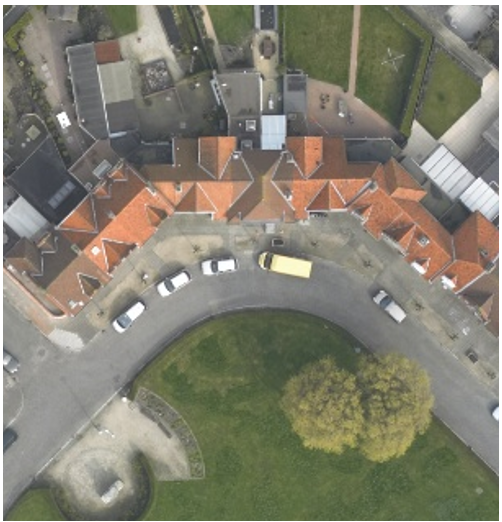
\includegraphics[height=2.0cm]{imgs/article/fig1a_zeebruges_image_aerienne}
      \legende{(a) aerial image}
    \end{minipage}\hspace{3mm}%
    \begin{minipage}[t]{0.22\textwidth}\centering
      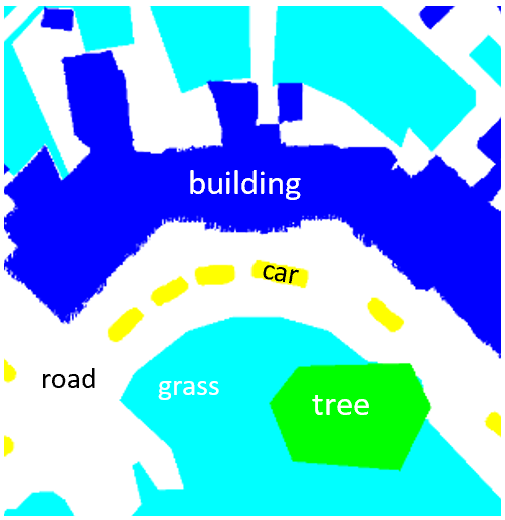
\includegraphics[height=2.0cm]{imgs/article/fig1b_zeebruges_carte_segmentation}
      \legende{(b) segmentation map}
    \end{minipage}}
  \credit{\emph{Zeebruges} dataset, IEEE GRSS IADF Technical Committee;
    imagery and ground truth: Belgian Royal Military Academy and ONERA.}
  \biblio{duda1973pattern,swain1978remote,richards1986remote}
\end{frame}

\begin{frame}{What sets remote sensing apart}
  \begin{itemize}
    \item Heterogeneous \hl{sensors}: optical, synthetic aperture radar (SAR),
          LiDAR.
    \item Variable spatial and spectral \hl{resolutions}; \hl{multitemporal} and
          \hl{multimodal} acquisitions.
    \item \hl{Complex geographical scenes} whose properties vary with region, season
          and acquisition conditions.
    \item The field is therefore not a simple adaptation of computer vision: it combines
          \hl{statistical pattern recognition}, \hl{signal processing},
          \hl{probabilistic modeling} and \hl{deep learning}.
  \end{itemize}
\end{frame}

\begin{frame}{Storyline}
  \formulebox{$I : \Omega \longrightarrow \mathbb{R}^{d}
              \qquad\text{then}\qquad
              f : \Omega \longrightarrow \mathcal{C}$}
  \begin{itemize}
    \item $\Omega$: the image domain; $d$: variables derived from spectral bands,
          SAR polarizations, LiDAR measurements, indices, DTMs, etc.
    \item $\mathcal{C}$: the finite set of semantic classes.
    \item The history of the field can be read as a \hl{progressive integration} of
          spectral, spatial, contextual and then multimodal information.
  \end{itemize}
  \vspace{0.4ex}
  \filrouge
\end{frame}

% ============================================================
\section{From pixel to context}
% ============================================================

\begin{frame}{The first approaches: per-pixel}
  \begin{itemize}
    \item In the late 1970s: Landsat (optical) and SeaSat (radar) create the need for
          automatic land-cover
          maps\refc{schowengerdt2007remote}\refc{landgrebe2003signal}\refc{ulaby2015microwave}
    \item Each pixel is an observation vector
          $\mathbf{x} = (x_1,\dots,x_d)^{\mathsf{T}}$: radiometric responses,
          SAR intensities, indices, ancillary data\refc{duda1973pattern}.
  \end{itemize}
  \formulebox{$\hat{\omega} \;=\; \arg\max_{\omega_i}\; P(\omega_i \mid \mathbf{x})$}
  \begin{itemize}
    \item Under a multivariate Gaussian assumption: the \hl{MAP classifier},
          \enquote{maximum a posteriori}, the reference method for several
          decades\refc{swain1978remote}\refc{richards1986remote}\refc{mather2004computer}
  \end{itemize}
  \biblio{duda1973pattern,swain1978remote,richards1986remote,schowengerdt2007remote,landgrebe2003signal,ulaby2015microwave,mather2004computer}
\end{frame}

\begin{frame}{Two limitations: dimensionality and independence}
  \begin{columns}[T,onlytextwidth]
    \begin{column}{0.50\textwidth}
      \begin{itemize}
        \item \hl{Curse of dimensionality} (Hughes
              phenomenon)\refc{hughes1968mean}: more variables do not guarantee
              better performance when few samples are available.
        \item \hl{Independence assumption on the observations}: each pixel is decided
              in isolation, without using its neighborhood, yet geographical objects are
              strongly spatially correlated: agricultural fields, forests, urban areas,
              road networks
        \item Consequence: \hl{noisy maps}, all the more so as spatial resolution
              increases
      \end{itemize}
    \end{column}
    \begin{column}{0.48\textwidth}\centering
      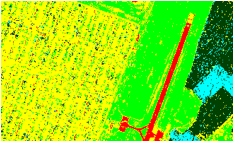
\includegraphics[width=0.72\textwidth]{imgs/article/fig2b_classification_pixel_a_pixel}
      \legende{Per-pixel classification: the salt-and-pepper effect\refc{moser2013landcover}}
    \end{column}
  \end{columns}
  \biblio{hughes1968mean,moser2013landcover}
\end{frame}

\begin{frame}{Discriminative and ensemble methods}
  \begin{itemize}
    \item From the late 1990s: estimating \hl{the decision boundaries
          directly}, rather than the distribution of the observations.
    \item \hl{SVMs}: margin maximization; good generalization in high
          dimension\refc{vapnik1998statistical}\refc{cortes1995support}\refc{campsvalls2009kernel}\refc{mountrakis2011support}.
    \item \hl{Kernels}: nonlinearity without losing convexity; many developments
          for geospatial observations\refc{scholkopf2002learning}.
    \item \hl{Random forests}: a vote of decision trees learned on random
          subsets; robustness, little tuning, variable
          importance\refc{breiman2001random}\refc{gislason2006random}.
    \item But these methods remain \hl{essentially per-pixel} classifiers
          when they are applied to local observations.
  \end{itemize}
  \biblio{vapnik1998statistical,cortes1995support,scholkopf2002learning,campsvalls2009kernel,mountrakis2011support,breiman2001random,gislason2006random}
\end{frame}

\begin{frame}{The contribution of spatial context}
  \begin{columns}[T,onlytextwidth]
    \begin{column}{0.32\textwidth}\centering
      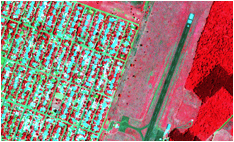
\includegraphics[width=0.84\textwidth]{imgs/article/fig2a_ikonos_fausses_couleurs}
      \legende{(a) IKONOS image}
    \end{column}
    \begin{column}{0.32\textwidth}\centering
      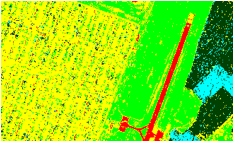
\includegraphics[width=0.84\textwidth]{imgs/article/fig2b_classification_pixel_a_pixel}
      \legende{(b) per-pixel}
    \end{column}
    \begin{column}{0.32\textwidth}\centering
      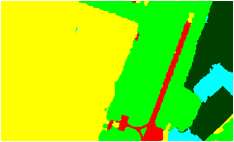
\includegraphics[width=0.84\textwidth]{imgs/article/fig2c_classification_contextuelle}
      \legende{(c) contextual}
    \end{column}
  \end{columns}
  \credit{IKONOS image, 4~m, 3 bands, false-color composite; segmentation
    maps \cite{moser2013landcover}.}
  \begin{itemize}
    \item In remote sensing, geographical objects exhibit \hl{strong spatial
          consistency}: fields, forests, urban areas, road networks.
    \item Labels must be estimated \hl{jointly}, not one pixel at a time.
  \end{itemize}
  % The French version cites `haralick1985image` here as well. That key is not
  % in the short bibliography, so the French slide prints a broken
  % "[haralick1985image] haralick1985image" line — a defect kept there only
  % because that version has to reproduce Martina Pastorino's PDF exactly.
  % Here the citation is simply dropped: the slide cites it nowhere else, and
  % reinstating the entry would shift every following [n] number.
  \biblio{richards1986remote,solberg1996markov,moser2013landcover}
\end{frame}

% ============================================================
\section{Markov and Bayesian models}
% ============================================================

\begin{frame}{Markov random fields: the first formalization}
  \begin{itemize}
    \item Labels become random variables defined on a \hl{neighborhood
          graph}\refc{geman1984stochastic}\refc{besag1986statistical}\refc{kato2012markov}.
    \item Under the Markov assumptions and the equivalence with Gibbs distributions,
          MAP estimation becomes an \hl{energy minimization}.
  \end{itemize}
  \formulebox{$\hat{Y} \;=\; \arg\max_{Y} P(Y \mid X)
              \qquad\Longleftrightarrow\qquad
              \hat{Y} \;=\; \arg\min_{Y} U(Y \mid X)$}
  \begin{itemize}
    \item $X$: the observations; $Y$: the label map to be estimated.
    \item MRFs provide a general framework linking local data and spatial
          consistency.
  \end{itemize}
  \biblio{geman1984stochastic,besag1986statistical,kato2012markov}
\end{frame}

\begin{frame}{Data term + regularization}
  \formulebox{$U(Y \mid X) \;=\; U_d(Y \mid X) \;+\; \beta\, U_r(Y \mid X)$}
  \begin{columns}[T,onlytextwidth]
    \begin{column}{0.56\textwidth}
      \begin{itemize}
        \item $U_d$: the \hl{data term}, derived from the likelihood.
        \item $U_r$: \hl{spatial regularization}, promoting consistency between
              neighboring pixels.
        \item $\beta$: the trade-off between fidelity and regularity.
        \item 1\textsuperscript{st}- or 2\textsuperscript{nd}-order neighborhoods; clique
              potentials \hl{penalize class changes} between
              \hl{adjacent pixels}\refc{kato2012markov}
      \end{itemize}
    \end{column}
    \begin{column}{0.42\textwidth}\centering
      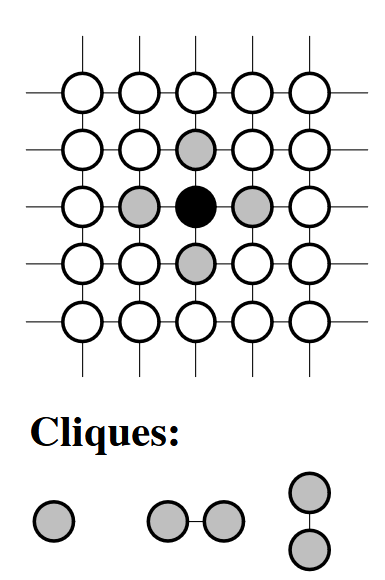
\includegraphics[height=2.5cm]{imgs/article/fig3a_voisinage_ordre1_cliques}%
      \hspace{2mm}%
      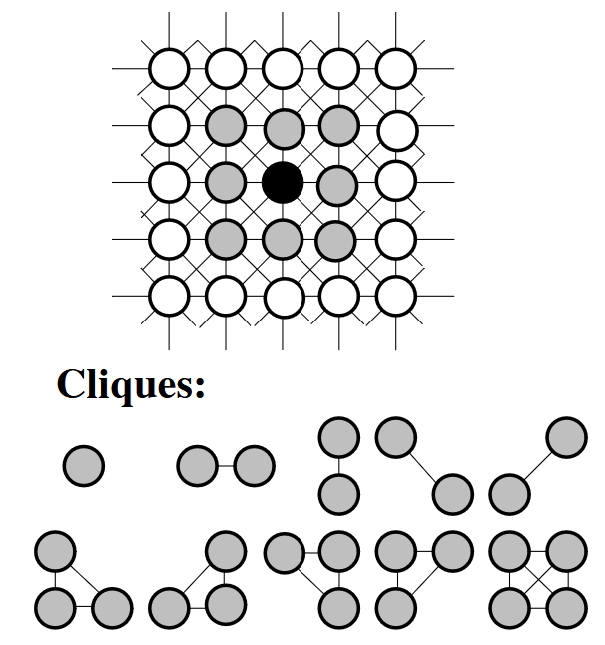
\includegraphics[height=2.5cm]{imgs/article/fig3b_voisinage_ordre2_cliques}
      \legende{(a) 1\textsuperscript{st} order \quad (b) 2\textsuperscript{nd} order}
      \credit{Pixel neighborhoods on a grid and the associated
        cliques \cite{kato2012markov}.}
    \end{column}
  \end{columns}
  \biblio{kato2012markov}
\end{frame}

\begin{frame}{Optimization and uses of MRFs}
  \begin{itemize}
    \item Finding the optimal configuration is a hard combinatorial optimization
          problem.
    \item Strategies: \hl{ICM}, \hl{simulated annealing}\refc{kirkpatrick1984optimization},
          the \hl{Gibbs sampler}\refc{geman1984stochastic},
          \hl{graph cuts}\refc{boykov2001fast}, loopy belief
          propagation\refc{tanaka2003loopy}.
    \item Applications: contextual classification, multisource segmentation,
          restoration, change detection, optical / radar /
          LiDAR fusion\refc{solberg1996markov}\refc{derin1987modeling}\refc{moser2013combining}.
    \item Beyond these applications: a \hl{general probabilistic formulation} of
          spatial regularization.
  \end{itemize}
  \biblio{geman1984stochastic,solberg1996markov,kirkpatrick1984optimization,boykov2001fast,tanaka2003loopy,derin1987modeling,moser2013combining}
\end{frame}

\begin{frame}{From MRFs to CRFs: a bridge to deep learning}
  \begin{itemize}
    \item Conditional random fields model $P(Y \mid X)$ directly rather than the joint
          distribution\refc{lafferty2001conditional}: this makes
          \hl{complex discriminative features} easier to use.
    \item \hl{Fully connected CRFs}: better preserved object
          boundaries\refc{krahenbuhl2011efficient}.
    \item Integration into deep networks: refinement modules, \hl{differentiable
          layers}\refc{zheng2015conditional}; hierarchical Markov frameworks
          and learned CRFs\refc{pastorino2021multisensor}\refc{pastorino2022semantic}\refc{pastorino2024crfnet}\refc{voisin2013classification}.
    \item \hl{The idea that runs through the field}: a map must be consistent both with
          the local observations \emph{and} with the spatial organization of the scene.
  \end{itemize}
  \biblio{lafferty2001conditional,krahenbuhl2011efficient,zheng2015conditional,pastorino2021multisensor,pastorino2022semantic,pastorino2024crfnet,voisin2013classification}
\end{frame}

% ============================================================
\section{Spectral-spatial and variational representations}
% ============================================================

\begin{frame}{Enriching the representation, not only the labels}
  \begin{itemize}
    \item Contextual models regularize the \hl{labels}; spectral-spatial methods
          enrich the \hl{features} before
          classification\refc{landgrebe2003signal}
    \item As resolutions increase, radiometric signatures alone become
          insufficient.
    \item Texture, shape, size, spatial organization and neighborhood relations
          become \hl{as discriminative as the spectral values
          themselves}\refc{dellepiane1991sar}.
    \item This rationale paves the way for the multiscale representations learned by
          deep networks\refc{blaschke2010object}.
  \end{itemize}
  \biblio{landgrebe2003signal,blaschke2010object,dellepiane1991sar}
\end{frame}

\begin{frame}{Mathematical morphology and multiscale profiles}
  \begin{columns}[T,onlytextwidth]
    \begin{column}{0.32\textwidth}\centering
      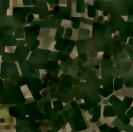
\includegraphics[height=2.15cm]{imgs/article/fig4a_erosion}
      \legende{erosion}
    \end{column}
    \begin{column}{0.32\textwidth}\centering
      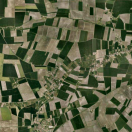
\includegraphics[height=2.15cm]{imgs/article/fig4b_image_originale_rvb}
      \legende{original RGB image}
    \end{column}
    \begin{column}{0.32\textwidth}\centering
      
\includegraphics[height=2.15cm]{imgs/article/fig4c_dilatation}
      \legende{dilation}
    \end{column}
  \end{columns}
  \credit{Erosion and dilation of the original RGB satellite image.}
  \begin{itemize}
    \item Operators: erosion, dilation, openings,
          closings\refc{serra1982image}\refc{soille2003morphological}.
    \item \hl{Extended morphological profiles} and \hl{attribute profiles} describe
          shape, size and contrast at several
          scales\refc{benediktsson2005classification}\refc{dallamura2010morphological}\refc{fauvel2008spectral}.
  \end{itemize}
  \biblio{serra1982image,soille2003morphological,benediktsson2005classification,dallamura2010morphological,fauvel2008spectral}
\end{frame}

\begin{frame}{Variational methods: regularizing the solution}
  \begin{itemize}
    \item A complementary approach: integrating spatial consistency directly into the
          formulation of the problem.
    \item Segmentation is formulated as an \hl{energy minimization} combining fidelity to
          the observations with spatial or geometric
          regularity \refc{samson2000variational}.
  \end{itemize}
  \formulebox{$E(u) = \text{data fidelity} +
              \lambda\,\text{spatial/geometric regularity}$}
  \begin{itemize}
    \item The \hl{Mumford--Shah} functional is one of the founding
          models\refc{mumford1989optimal}.
    \item The principles of data/regularity trade-off, multiscale analysis and fusion will
          reappear in learned forms in deep learning.
  \end{itemize}
  \biblio{mumford1989optimal,samson2000variational}
\end{frame}

% ============================================================
\section{Deep learning and foundation models}
% ============================================================

\begin{frame}{Going deep}
  \begin{columns}[T,onlytextwidth]
    \begin{column}{0.52\textwidth}
      \begin{itemize}
        \item 2012, the turning point: \hl{AlexNet} demonstrates a dramatic improvement in
              natural-image classification\refc{krizhevsky2012imagenet}
        \item The change: learning the representations and the decision function jointly,
              directly from the data.
        \item \hl{FCNs}: dense, pixel-level prediction.
      \end{itemize}
    \end{column}
    \begin{column}{0.43\textwidth}\centering
      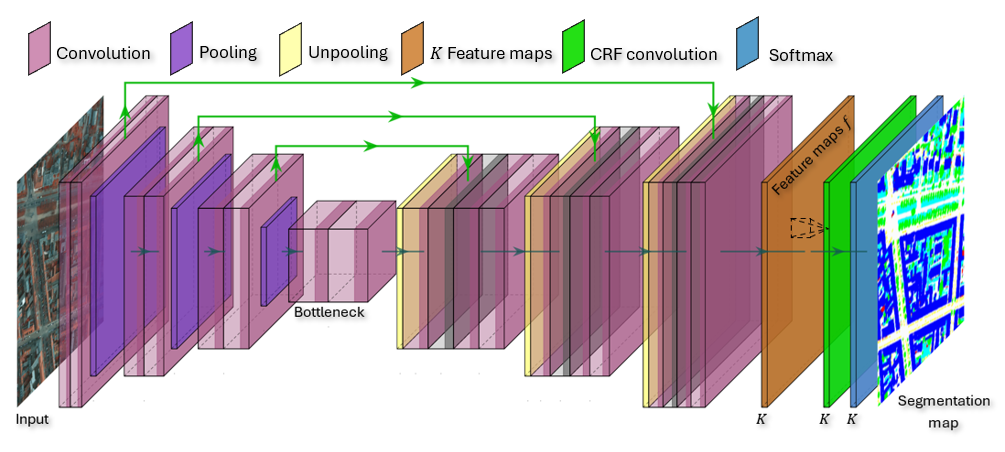
\includegraphics[width=0.95\textwidth]{imgs/article/fig6_fcn_potsdam}
      \legende{FCN architecture applied to Potsdam}
    \end{column}
  \end{columns}
  \vspace{1.2ex}
  \begin{itemize}
    \item \hl{U-Net}: skip connections to restore spatial information.
    \item \hl{DeepLab}: dilated convolutions and multiscale representations to enlarge
          the receptive field.
  \end{itemize}
  \biblio{krizhevsky2012imagenet,long2015fully,ronneberger2015unet,chen2018encoder,audebert2018beyond,ma2019deep}
\end{frame}

\begin{frame}{Transformers, self-supervision and foundation models}
  % Columns without `onlytextwidth`: the block slightly overflows the text margins,
  % which leaves room for figure 7 (the widest in the presentation).
  \begin{columns}[T]
    \begin{column}{0.58\textwidth}
      \begin{itemize}
        \item CNNs remain limited by the need for annotations and by the modeling of
              long-range dependencies.
        \item \hl{Attention} mechanisms and transformers better represent the
              interactions between distant
              regions\refc{vaswani2017attention}\refc{dosovitskiy2021image}.
        \item \hl{Self-supervision} exploits large volumes of unlabeled satellite images
              to learn transferable
              representations\refc{he2022masked}.
      \end{itemize}
    \end{column}
    \begin{column}{0.41\textwidth}\centering
      \vspace{1.65ex}
      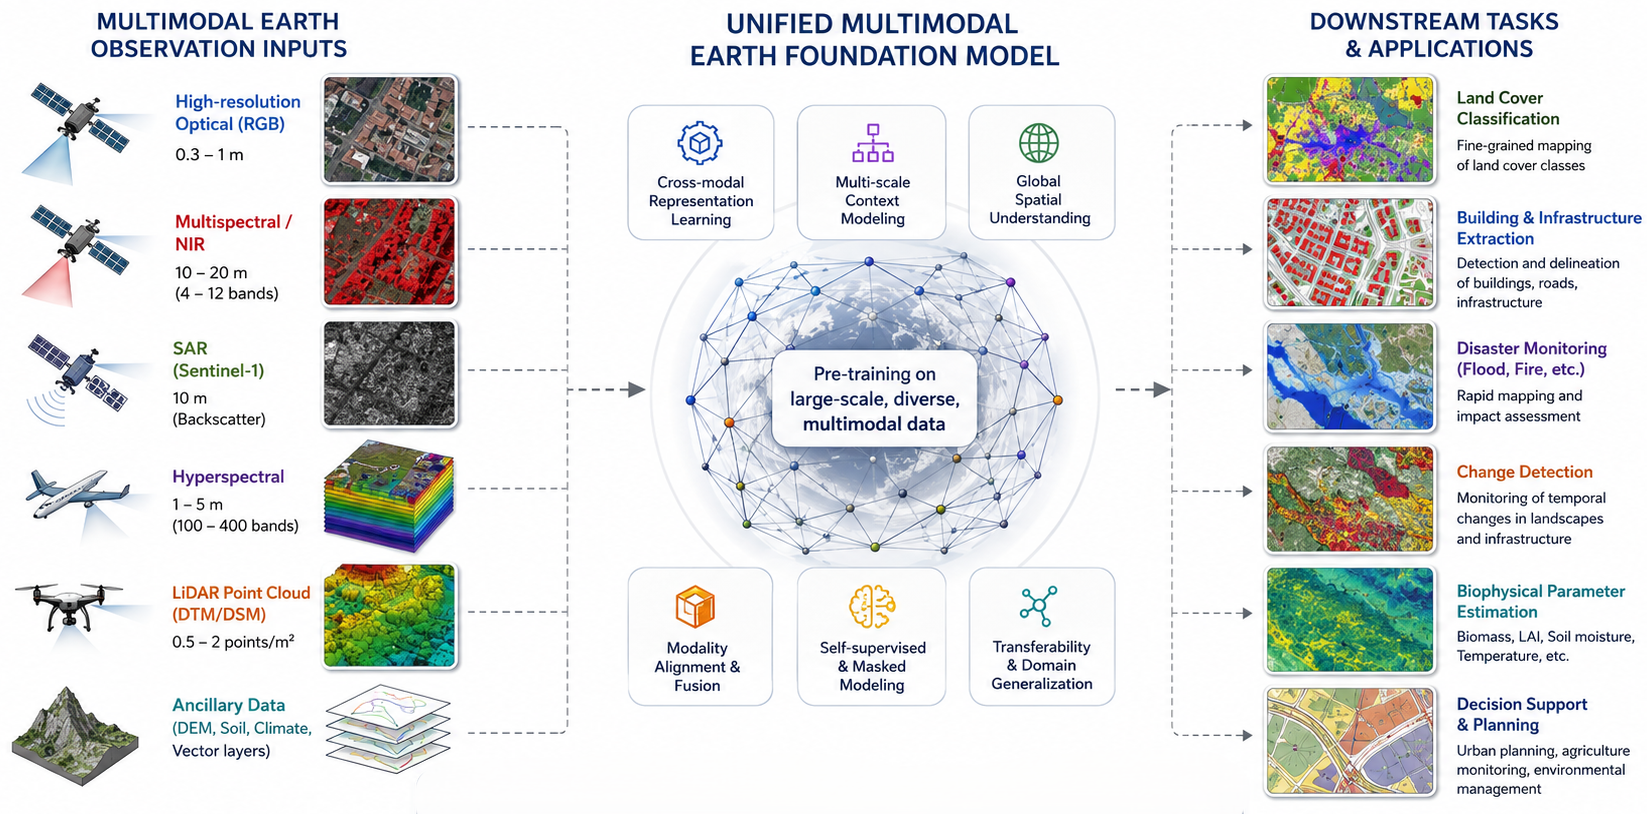
\includegraphics[width=\textwidth]{imgs/article/fig7_modele_fondation_geospatial}
      \legende{Principle of a geospatial foundation model}
    \end{column}
  \end{columns}
  \begin{itemize}
    \item The goal: moving from a specialized model to \hl{general, multimodal and
          transferable representations (geospatial foundation
          models)}\refc{xiao2025foundation}.
  \end{itemize}
  \biblio{vaswani2017attention,dosovitskiy2021image,he2022masked,xiao2025foundation}
\end{frame}

% ============================================================
\section{Open challenges}
% ============================================================

\begin{frame}{Open challenges}
  \begin{itemize}
    \item \hl{Generalization} across regions, seasons, sensors and resolutions.
    \item \hl{Lack of annotations}: high cost of ground-truth data, class imbalance,
          noisy labels.
    \item \hl{Multimodal fusion}: optical, SAR, LiDAR, time series and ancillary
          data.
    \item \hl{Robustness}: distribution shift, clouds, noise, artifacts, rare
          events.
    \item \hl{Interpretability}: understanding and controlling the decisions of
          increasingly large models.
  \end{itemize}
\end{frame}

\begin{frame}{Conclusion: a nonlinear history}
  \begin{itemize}
    \item Not a simple trajectory from statistical classifiers to deep networks, but
          the \hl{convergence of several families of methods}: statistical
          classification, kernel methods, ensemble methods, contextual models,
          Markov random fields, variational methods, stochastic geometry, deep
          learning, foundation models
    \item One unifying reading: the \hl{progressive integration of increasing levels of
          context}
  \end{itemize}
  \vspace{0.6ex}
  \filrouge
  \vspace{0.4ex}
  \begin{itemize}
    \item One recurring principle: \hl{data term $+$ regularization},
          from Markov random fields to the loss functions of deep networks
  \end{itemize}
\end{frame}

% ---- Thank you ---------------------------------------------
\frame{\merci}

% ============================================================
% Appendix: full bibliography
% ============================================================
\begin{frame}[allowframebreaks]{References}
  \printbibliography[heading=none]
\end{frame}

\end{document}
